\documentclass[a4paper, 12pt,oneside]{article} 
%\documentclass[a4paper, 12pt,oneside,draft]{article} 
\usepackage{preamble}
%--------------------- ACTUAL FILE ---------------------- %
\begin{document} 
%%%
	%\setcounter{page}{1}
	\begin{center}
	    \Large
	    \textbf{How and When to Use Hamiltonian Monte Carlo} 
	    \vspace{0.4cm}
	    \large

		Course : Stochastic Simulation \\
	    Students : Aude Maier \& Tara Fjellman \\
	    \small{Fall 2024}
	\end{center}

	\section{Introduction}
	\section{Core Theory}
		\subsection{RWMC}
		\subsection{HMC}
			\subsubsection{The Algorithm}
			\subsubsection{Acceptance Rate}
			\subsubsection{Convergence to Target Distribution}
	\section{(c)}
        \subsection{Gibbs distribution invariance}
		Under the assumption that there is no numerical error, we want to prove that the Gibbs measure is invariant for the chain generated by the hamiltonian dynamics.

		This is equivalent to saying that the Gibbs measure $\pi$ is the same before and after an evolution of $t$ seconds from the hamiltonian dynamics. 
		To prove this we first introduce hamiltonian dynamics operators $\phi,\Phi$ acting respectively on the phase space and the Gibbs measure : $\phi_t(q_s,p_s)=(q_{s+t},p_{s+t});\Phi_t[\pi_s]=\pi_{t+s}\quad \forall t\in\mathbb{R}$.
		The statement we want to prove can then be expressed as 
		\begin{gather}
			\Phi_t[\pi_s](D)=\pi_{s+t}(D)\quad \forall D\in\mathcal{B}(\Omega),\forall s,t\in\mathbb{R},
			%P(T_t(q,p)\in D_s)=
			%P((q,p)\in T_{-t}(D_s))=
			%P((q,p)\in D_s)=\pi(D_s),
			%P((q,p))=\int_{\Omega} K((q,p),D_s) G(q,p) \ dq dp=\pi(T_t[D_s]),
		\end{gather}
		with $\Omega$ the phase space.

		We can now write the left hand side of the equation as
		\begin{align}
			\Phi_t[\pi_s](D)&=\int_D \pi_{s+t}(q,p)\ dqdp \\
				&=\int_{\phi_{-t}(D)}\pi_{s}(q,p)\ dqdp \\
				&=\pi_s(\phi_{-t}(D)).
		\end{align}
		The final result is obtained using the fact that volumes in phase space are preserved by the hamiltonian dynamics (in conservative systems). This result is known as Liouville's theorem, but is mentioned as theorems 2.3 in [cite].
		%K:\Omega \times D\to [0,1]$ the transition kernel of the chain, $G(q,p)$ the Gibbs distribution, and $T_t[\cdot]$ the hamiltonian time evolution operator defined by $T[(q_s,p_s)]=(q_{s+t},p_{s+t})$.

		This implies specifically that $q_k\sim\pi$ for all $k\in\mathbb{N}$ if $q_0\sim \pi$. 

		If the dynamics is discretised with the Velocity Verlet algorithm, the volume in phase space is preserved up to a small error, which is why the algorithm is used in practice [cite wikipedia]. 
        \subsection{What happens for discrete evolution ?}
	\section{Exploring a 2D example}
		\subsection{Context}
		\lipsum[1]
        \begin{figure}[htb]
            \centering
                \vspace{0em}
                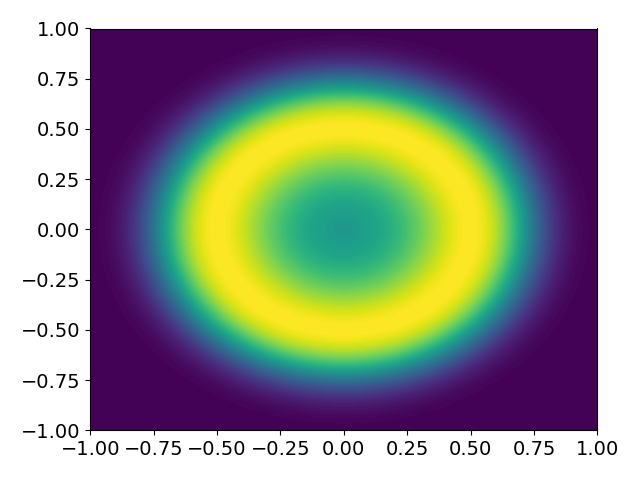
\includegraphics[width=0.6\textwidth]{density_alpha=10}
                \caption{Hello there.}
                \label{fig:density-alpha=10}
        \end{figure}
		\subsection{RWMC Solution}
        \begin{figure}[htb]
            \centering
                \vspace{0em}
                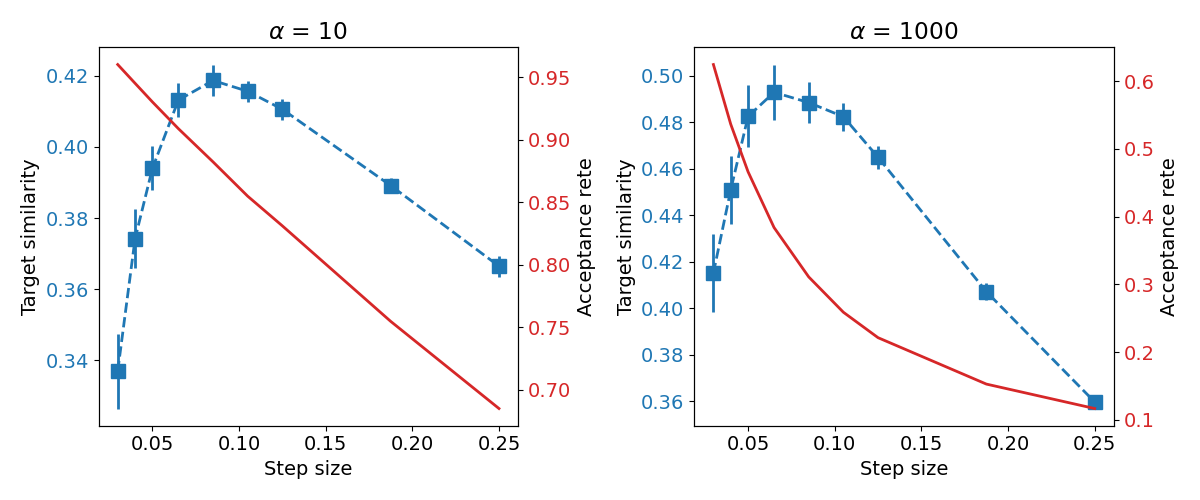
\includegraphics[width=0.95\textwidth]{rwmc_scan}
                \caption{Similarity as a function of RWMC step size for considered values of $\alpha$.}
                \label{fig:rwmc-scan}
        \end{figure}
		\lipsum[1]
		\subsection{HMC Solution}
		\begin{wrapfigure}[18]{r}{0.6\textwidth}
			\centering
				\vspace{-2em}
				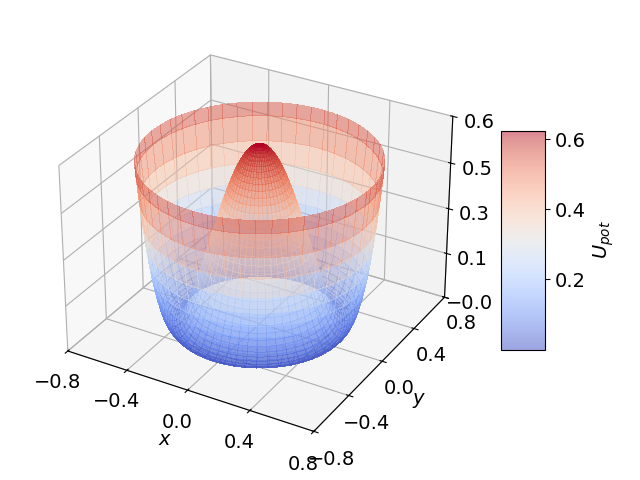
\includegraphics[width=0.57\textwidth]{U_pot_alpha=10}
				\caption{Potential energy landscape associated to HMC algorithm for $\alpha=10$. Version for $\alpha=1000$ is identical, except scales are scaled by a factor of 100.}
				\label{fig:U-pot-alpha=10}
		\end{wrapfigure}
		\lipsum[1]
			\subsubsection{Impact of Integration Time}
			\begin{figure}[htb]
				\centering
					\vspace{0em}
					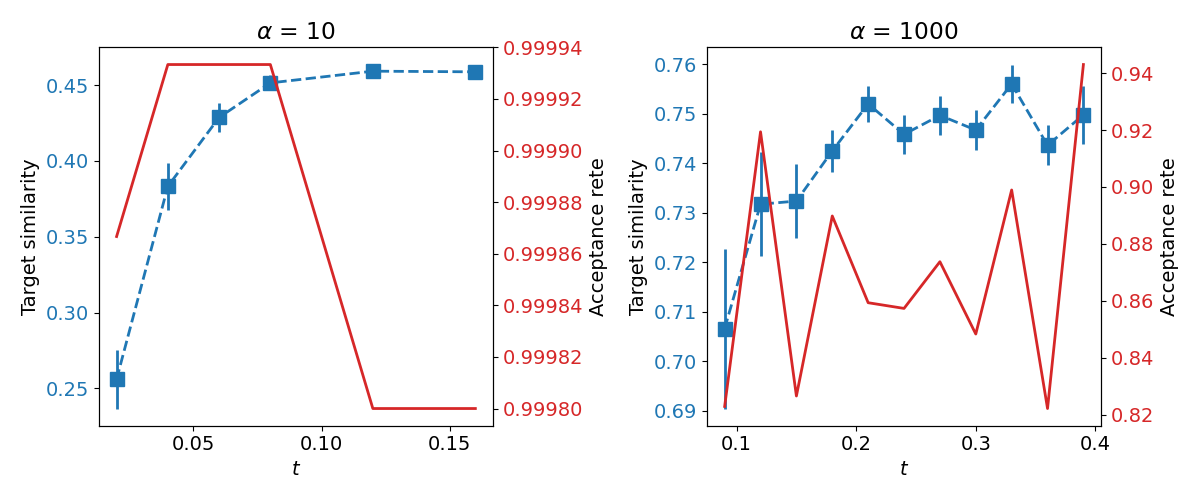
\includegraphics[width=0.95\textwidth]{t_scan}
					\caption{Similarity as a function of HMC integration time for considered values of $\alpha$.}
					\label{fig:t-scan}
			\end{figure}
			\lipsum[1]
			\subsection{Impact of $\Delta t$}
			\begin{figure}[htb]
				\centering
					\vspace{0em}
					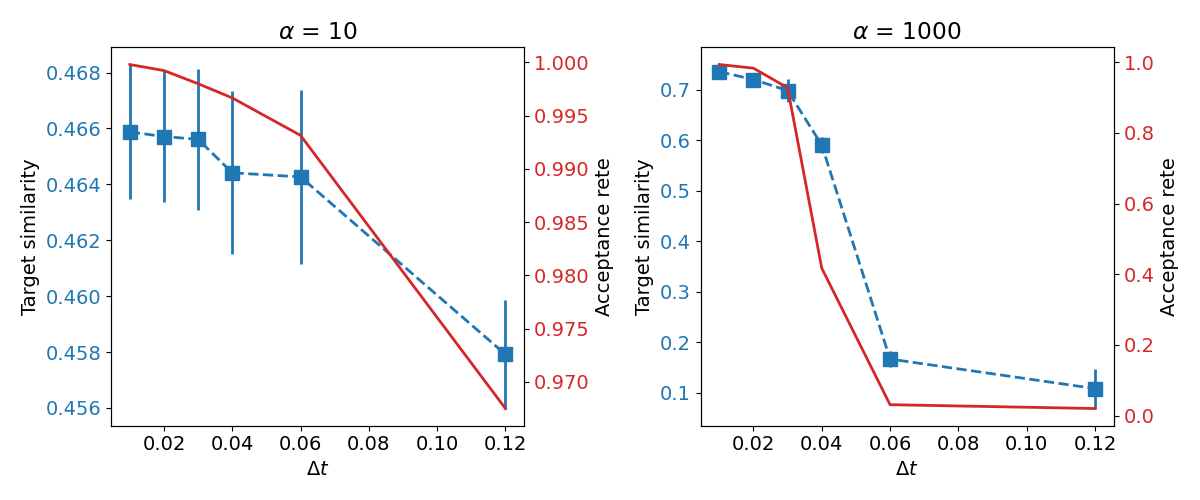
\includegraphics[width=0.95\textwidth]{dt_scan}
					\caption{Similarity as a function of HMC time step for considered values of $\alpha$.}
					\label{fig:dt-scan}
			\end{figure}
			\lipsum[1]
			\subsection{Impact of Mass Scale}
			\begin{figure}[htb]
				\centering
					\vspace{0em}
					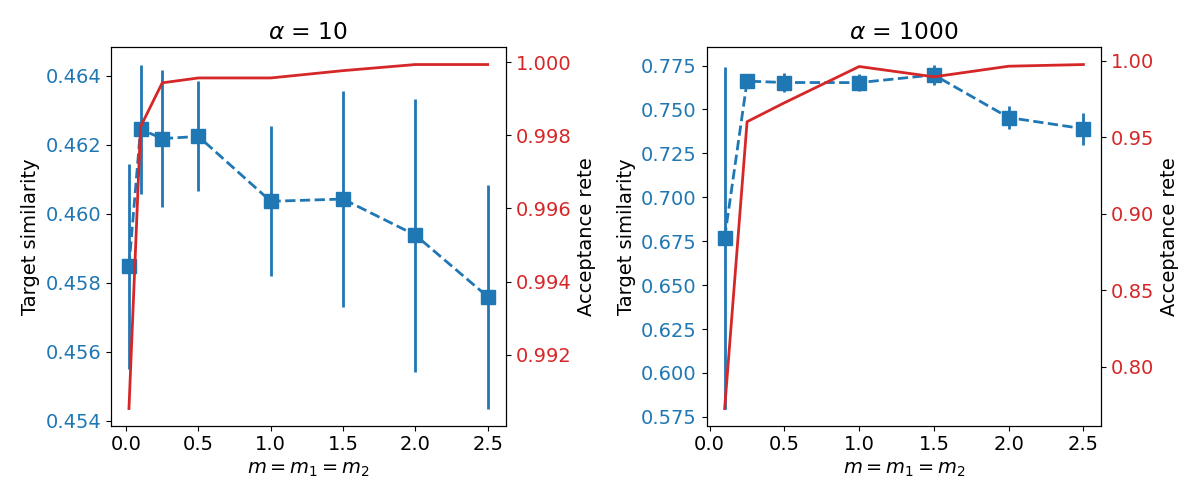
\includegraphics[width=0.95\textwidth]{mass_scan}
					\caption{Similarity as a function of HMC mass scale for considered values of $\alpha$.}
					\label{fig:mass-scan}
			\end{figure}
			\lipsum[1]
			\subsection{Impact of Mass Symmetry}
			\begin{figure}[htb]
				\centering
					\vspace{0em}
					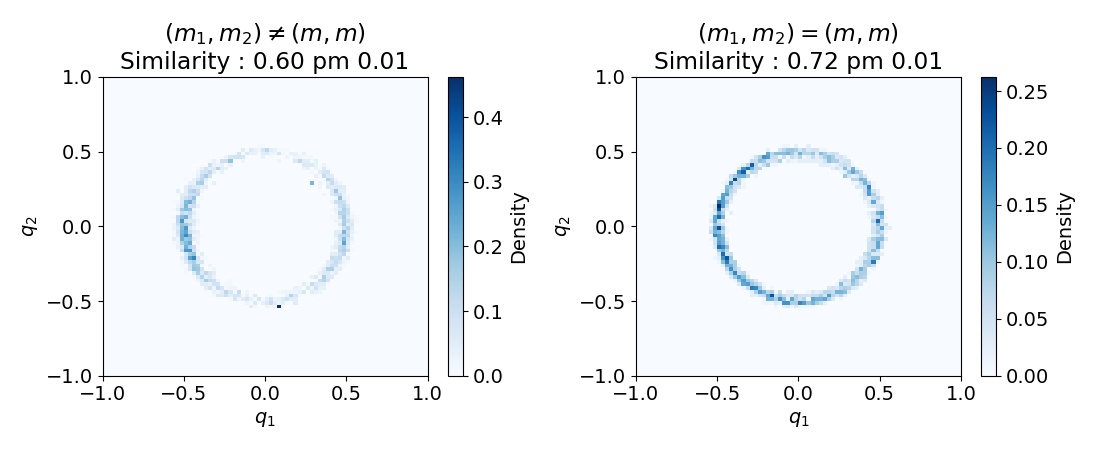
\includegraphics[width=0.95\textwidth]{mass_sym}
					\caption{Similarity for HMC samplers with asymmetric and symmetric masses for $\alpha=1000$.}
					\label{fig:mass-sym}
			\end{figure}
			\lipsum[1]
		\subsection{Comparison and Sample-Size Evolution}
		\begin{figure}[htb]
			\centering
				\vspace{0em}
				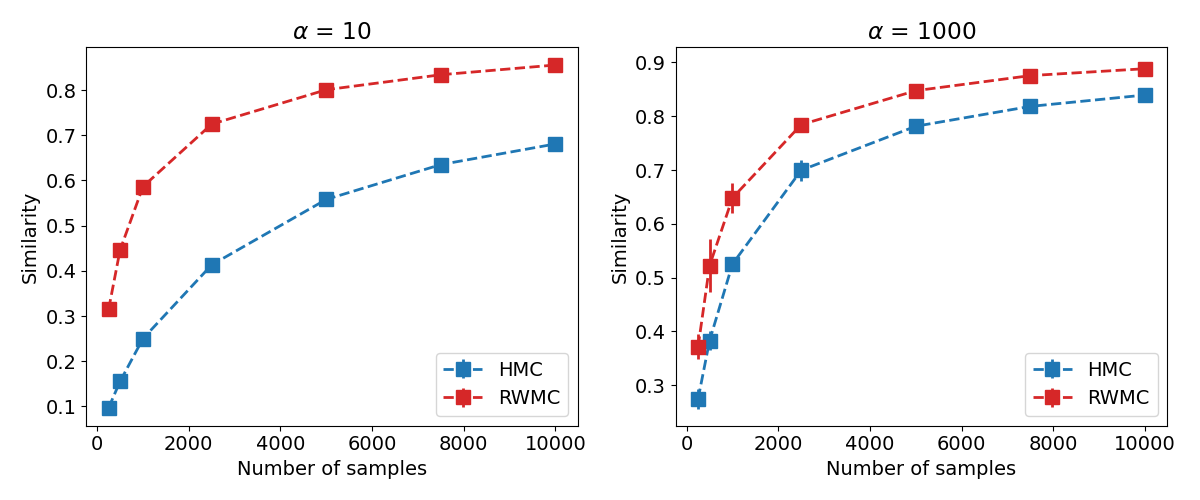
\includegraphics[width=0.95\textwidth]{nsamples_evolution}
				\caption{Similarity as a function of sample-size for RWMC and HMC samplers and considered values of $\alpha$. The sample-size represented on the x axis is that associated to the HMC sampler. The associated RWMC sample-size is obtained by matching the number of function evalutations of the HMC sampler.}
				\label{fig:nsamples-evolution}
		\end{figure}
		\lipsum[1]
	\section{US Birthweight Data}
		\subsection{HMC Solution}
		\subsection{RWMC Solution}
	\section{(f)}
	As an alternative to HMC we consider rejection sampling. We therefore want to find a function $g(q)$ and a constant $C$ such that the following inequality holds for all $q$:
	\begin{equation}
		\tilde{f}(q) = e^{q^TX^T(y-1_{n})}e^{-1_{n}^T \log[1+\exp(-x_i^Tq)]_{n\times 1}}e^{-\frac{1}{2}q^T\Sigma^{-1} q} \leq Cg(q),
	\end{equation}
	where we have denoted $\Sigma=\text{Diag}(\sigma_1^2,...,\sigma_p^2)$.
	Given that 
	\begin{equation}
		\log[1+\exp(-x_i^Tq)] \le \log(2) - x_i^Tq,
	\end{equation}
	\begin{equation}
		e^{-\sum_i \log[1+\exp(-x_i^Tq)]} = \prod_i \frac{1}{1+\exp(-x_i^Tq)}<1,
	\end{equation}
	we can simplify the problem to finding a function $g(q)$ such that
	\begin{equation}
		\tilde{f}(q) \le 2^{-n}e^{-q^TX^T 1_n} e^{q^TX^T(y-1_{n})}e^{-\frac{1}{2}q^T\Sigma^{-1} q} = 2^{-n}e^{q^Tb}e^{-\frac{1}{2}q^T\Sigma^{-1} q}
		=: Cg(q),
	\end{equation}
	with $b=X^T(y-2_{n})$. 

	By completing the square in the exponent of $Cg(q)$, we can write it in terms of a Multivariate Gaussian distribution with mean $\mu=\Sigma b$ and covariance $\Sigma$. Indeed : 
	% TO DO : change into a double equality going from Cg(q) to clean expression in terms of completed square
	\begin{gather}
		%e^{q^Tb}e^{-\frac{1}{2}q^T\Sigma^{-1} q} = 
		e^{-\frac{1}{2}(q-\mu)^T\Sigma^{-1} (q-\mu)} =
		e^{-\frac{1}{2}\mu^T\Sigma^{-1}\mu}
		e^{q^T\Sigma^{-1}\mu}
		e^{-\frac{1}{2}q^T\Sigma^{-1} q} \\
		\implies \tilde{f}(q) \le 2^{-n}e^{\frac{1}{2}\mu^T\Sigma^{-1} \mu}e^{-\frac{1}{2}(q-\mu)^T\Sigma^{-1}(q-\mu)}.
	\end{gather}
	Using now the normalisation constant of the Multivariate Gaussian distribution 
	\begin{gather}
		\sqrt{(2\pi)^p|\Sigma|}=\int_{\mathbb{R}^p}e^{-\frac{1}{2}(q-\mu)^T\Sigma^{-1}(q-\mu)}\ dq,
	\end{gather} 
	we can define $g$ and $C$ as 
	\begin{gather}
		g(q)=\frac{1}{\sqrt{(2\pi)^p|\Sigma|}}e^{-\frac{1}{2}(q-\mu)^T\Sigma^{-1}(q-\mu)}, \\
		C = 2^{-n}e^{\frac{1}{2}\mu^T\Sigma^{-1} \mu}{\sqrt{(2\pi)^p|\Sigma|}} = 2^{-n}\sqrt{(2\pi)^p|\Sigma|e^{\mu^T\Sigma^{-1} \mu}}.
	\end{gather} 
	\section{Section ...}
	\section{Conclusion}
	\section*{Aknowledgements}
	\section*{References}
	%\appendix
	%	\section{Runtime Estimation}\label{appendix:runtime_estimation}
%%%
\end{document} 

